\documentclass[tikz,border=2pt,png]{standalone}
\usepackage{tkz-euclide}
\usetikzlibrary{intersections,decorations.markings}
\begin{document}
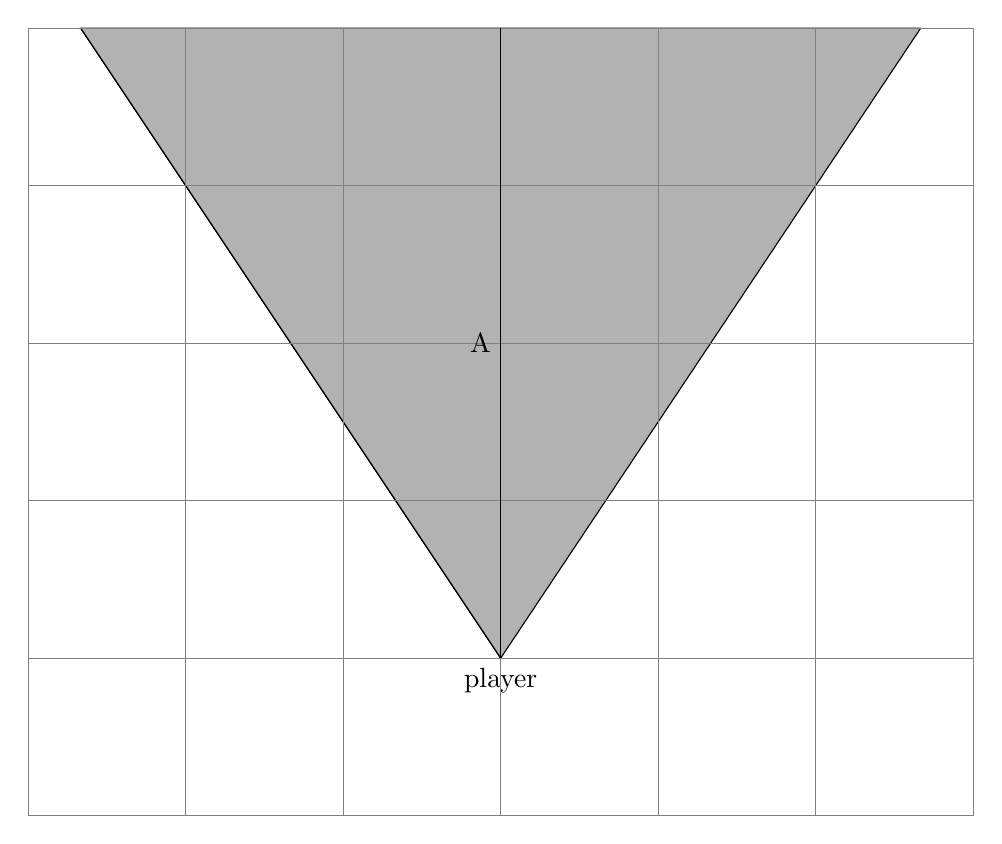
\begin{tikzpicture}[scale=2.0]


\newcommand\roomwidth{3}
\newcommand\roomheight{5}



  \draw (-\roomwidth,0) coordinate (O) -- (-\roomwidth,\roomheight) coordinate (wall0) --
        (\roomwidth,\roomheight) coordinate (wall1) -- (\roomwidth,0) coordinate (B);


\newcommand\playerx{0}
\newcommand\playery{1}

 \coordinate(player) at (\playerx,\playery);
\node[align=center, below] at (player) {player};

\newcommand\halfviewfield{4}
\newcommand\depthofview{7}

\coordinate(rightFrustrum) at player ++ (\halfviewfield,\depthofview);
\coordinate(leftFrustrum) at player ++ (-\halfviewfield,\depthofview);


%\fill[red] (intersection of player--leftFrustrum and wall0--wall1) circle (2pt); 
%\fill[red] (intersection of player--rightFrustrum and wall0--wall1) circle (2pt); 

\filldraw[fill=black!30!white, draw=black] (player) -- (intersection of player--leftFrustrum and wall0--wall1) -- (intersection of player--rightFrustrum and wall0--wall1);
\draw [draw=black](player) -- (intersection of player--leftFrustrum and wall0--wall1);
\draw [draw=black](player) -- (intersection of player--rightFrustrum and wall0--wall1);
% \draw [draw=black](player) -- (rightFrustrum);
% \draw [draw=black](player) -- (leftFrustrum);




\foreach \y in {0,...,\roomheight}
  \draw [draw=black!50!white] (-\roomwidth,\y) -- (\roomwidth,\y);

\foreach \x in {-\roomwidth,...,\roomwidth}
  \draw [draw=black!50!white] (\x,0) -- (\x,\roomheight);

\draw [draw=black](\playerx,\playery) -- (\playerx,\roomheight) node[pos=0.5,align=center, left]{A};

\end{tikzpicture}
\end{document}